%
%
%
%%%%%%%%%%%%%%%%%%%%%%%%%%%%%%%%%%%%%%%%%%%%%%%%%%%%%%%%%%%%%%%%%%%%%%%
%                           SUBSECTION                                %
%%%%%%%%%%%%%%%%%%%%%%%%%%%%%%%%%%%%%%%%%%%%%%%%%%%%%%%%%%%%%%%%%%%%%%%
%
%
%

\subsection{Сферические микрорезонаторы}

    Неотъемлемым элементом почти любого сложного оптического и микроволнового прибора является резонатор. Именно прогресс в совершенствовании резонаторов зачастую приводил к достижению качественно новых результатов. Так, появление мазеров и лазеров было бы невозможно без реализации высокодобротных резонаторов СВЧ и оптического диапазонов. Высокодобротные резонаторы активно используются для сужения и стабилизации линии генерации, в качестве фильтров и дискриминаторов, в разнообразных высокочувствительных сенсорах и датчиках, в метрологии и в прецизионных физических экспериментах. \cite{microresonators}

    Так, одним из ключевых направлений развития физики сегодня является квантовая теория измерений и связанный с ней интерес к манипуляциям с отдельными квантовыми объектами. Резонаторы играют существенную роль в этих исследованиях. Именно с помощью миниатюрных высокодобротных резонаторов в оптическом диапазоне были впервые продемонстрированы неклассические состояния электромагнитного поля и были впервые проведены впечатляющие эксперименты по наблюдению эффектов взаимодействия отдельных фотонов и отдельных атомов. Тесно связаны с этим направлением и такие, вызывающие активное внимание и ожидания, приложения, как квантовые компьютеры, квантовая криптография и квантовая телепортация. Одним из основных требований для наблюдения квантовых эффектов является изоляция системы от внешнего классического мира и уменьшение в ней диссипации для замедления распада состояний (декогеренции), что означает для резонаторов повышение добротности. \cite{microresonators}

    Взаимодействие излучения со сферическими телами исследуется уже более 100 лет. В последние десятилетия, в связи с обнаружением сверхузких резонансов рассеяния и возможностью создания на этой основе микрорезонаторов с гигантской добротностью, открывающих новые горизонты оптической микрофотоники, интерес к этому вопросу усилился многократно. \cite{microresonators}

    Повышенный интерес к микрорезонаторам и бурное развитие области сверхдобротных резонаторов ставят перед наукой и другие задачи. Всесторонний анализ различных путей диссипации энергии в микрорезонаторах с целью повышения их добротности и стабильности является задачей, требующей особого внимания. Для микроэлектронных приборов, элементов квантовых компьютеров и т.д. не менее важным является вопрос устранения шумов. Тепловые шумы являются довольно серьезным мешающим фактором. Генерация этих шумов на сферических микроструктурах тоже требует изучения в целях их учета и компенсации.

    На \autoref{fig:spherical_resonator} показан сферический микрорезонатор с МШГ (моды шепчущей галереи). В виде пояса видна спекл-картина рассеяния на поверхностных неоднородностях поля МШГ.
    %
    \begin{figure}[h]
        \centering
        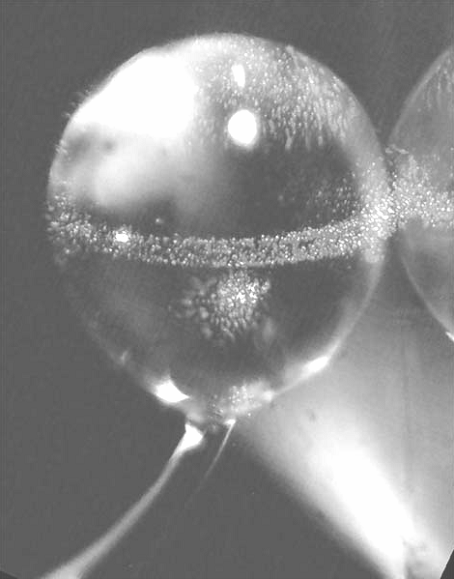
\includegraphics[width=0.5\textwidth]{spherical_resonator}
        \caption[]{Оптический сферический микрорезонатор на ножке рядом с возбуждающей призмой, в которой видно его отражение. Диаметр около $570$ мкм, добротность $> 10^9$. Физический факультет МГУ \cite{microresonators}}
        \label{fig:spherical_resonator}
    \end{figure}

%
%
%
%%%%%%%%%%%%%%%%%%%%%%%%%%%%%%%%%%%%%%%%%%%%%%%%%%%%%%%%%%%%%%%%%%%%%%%
%                           SUBSECTION                                %
%%%%%%%%%%%%%%%%%%%%%%%%%%%%%%%%%%%%%%%%%%%%%%%%%%%%%%%%%%%%%%%%%%%%%%%
%
%
%

\subsection{Модель сферического резонатора}

    В данной работе мы рассмотрим идеализированную модель сферического резонатора с идеально проводящими стенками. Хоть это в чистом виде и не выполняется на практике, такая идеализация позволит без лишних усложнений ввести основные понятия и продемонстрировать основные методики расчета дифференциальных и интегральных характеристик электромагнитного поля в системах со сферической симметрией.

    Форму резонатора будем полагать идеально сферической с радиусом $r_\text{шара}$. Стенки резонатора будем считать идеально проводящими. Также будем полагать, что резонатор заполнен диэлектриком, для которого выполняются линейные материальные соотношения (иными словами, среда изотропная и бездисперсионная).

%
%
%
%%%%%%%%%%%%%%%%%%%%%%%%%%%%%%%%%%%%%%%%%%%%%%%%%%%%%%%%%%%%%%%%%%%%%%%
%                           SUBSECTION                                %
%%%%%%%%%%%%%%%%%%%%%%%%%%%%%%%%%%%%%%%%%%%%%%%%%%%%%%%%%%%%%%%%%%%%%%%
%
%
%

\subsection{Цели работы}

    Изучение термодинамики сферических структур важно для современной микроэлектроники, оптики и других наук, оперирующих со сферически симметричными малоразмерными структурами. В частности, оно позволяет получить более или менее точные количественные оценки мешающих факторов~--- тепловых шумов, а также указать возможные способы компенсации их воздействия.

    В данной работы мы поставим для себя следующие цели:
    %
    \begin{enumerate}[nosep]
        \item описание электромагнитного поля внутри резонатора,
        \item описание спектральной плотности запасенной в резонаторе энергии.
    \end{enumerate}

    Для достижения первой цели мы предложим альтернативную методику построения мод электромагнитного поля и применим ее для описания поля в рассматриваемой системе.

    Классические методики решения данной задачи в значительной степени эвристичны, другие приводят к весьма громоздким результатам. К тому же их применение к полям б\'{о}льшей тензорной размерности весьма проблематично. \cite{burlankov_tmf}

    В данной работе приводится новый подход, в основе которого лежат векторы Киллинга пространства, в котором рассматривается поле. Данный подход учитывает естественную симметрию объемлющего пространства, тем самым требует более коротких выкладок. К тому же он естественным образом обобщается для описания полей любой тензорной размерности, например гравитационного. \cite{burlankov_tmf}

    Впервые указанная методика была применена для описания полей различной тензорной размерности на трехмерной сфере \cite{burlankov_tmf}.

    В последней части работы мы построим кривую спектральной плотности энергии, запасенной в резонаторе, через численный анализ набора собственных частот резонатора и количества соответствующих им мод. Мы покажем, что формула Планка асимптотически верна и в случае сферических резонаторов, причем даже в области достаточно низких частот расхождения не являются существенными.

    Поскольку предметом нашего рассмотрения является \textit{термодинамика}, мы будем считать, что энергия в резонатор поступает из окружающей среды за счет непрерывного теплообмена. Мы сразу будем полагать, что вся рассматриваемая система находится в состоянии термодинамического равновесия. Конкретный механизм теплообмена нас не интересует, однако указанные факты позволят нам применить известные законы статистической физики к описанию вероятностных характеристик нашей модели. Более того, в силу стохастического характера теплообмена в резонаторе не будет каких-либо выделенных мод.
